%!TEX root = ../notas_de_clase.tex

\section{Regresión No Lineal}
El concepto de regresión lineal puede ser extendido para representar relaciones no lineales entre variables de entrada y salida. Dicha extensión consiste en la aplicación de una transformación (de parámetros fijos) a la variable independiente, para luego aplicar un modelo, como los estudiados en el capítulo anterior, a la nueva variable transformada. 

Específicamente, consideraremos transformaciones a valores vectoriales de la variable independiente de la siguiente forma
\begin{align}
  \Phi \colon \R^M &\to \R^D \nonumber\\
  x &\mapsto \Phi(x)=[\phi_1(x),\ldots,\phi_D(x)]^\top
\end{align}
donde $\{ \phi_i \}_{j=1}^D$ son funciones escalares. 

\begin{mdframed}[style=discusion, frametitle={\center Observaciones}]

\noindent 1) Nos referiremos a $\Phi(x)$ como \emph{características} y a $x$ simplementes como \emph{datos crudos}. Esta notación está motivada por una representación de la variable independiente que es coherente o interpretable y por ende permite resolver el problema con un modelo de regresión simple e interpretable como el modelo lineal. Debido a su rol de conectar las partes lineales y no lineales del modelo, nos referiremos a $\Phi(\cdot)$ como la función de \emph{enlace}.\\

\noindent 2) En la práctica, la función $\Phi:x\mapsto\Phi(x)$ es elegida en base  al conocimiento \emph{experto} que se tenga del problema de regresión a resolver;  como su elección pretende extraer las características de interés y representarlas  de una forma compatible con el modelo lineal, entonces, nos referiremos a la construcción \emph{manual} de la función $\Phi$ como \emph{ingeniería de características}. \\

\noindent 3) La función $\Phi$ puede tener parámetros, elegidos manualmente por ahora. Sin embargo, más adelante veremos modelos donde los parámetros de $\Phi$ también pueden ser encontrados (e.g., mediante optimización). En dicho caso, es posible interpretar que la ingeniería dee features no es realizada de forma manual, sino que automatizada.  


\end{mdframed}

\subsection{Modelo lineal en los parámetros} 
\label{sub:modelo_lineal_param}


Usando el vector de características $\Phi(x)$ como entrada a un modelo lineal, podemos definir el siguiente modelo de regresión: 

\begin{equation}
    y = \theta^\top\Phi(x) + \epsilon,\quad \epsilon\sim\cN(0,\sigma_\epsilon^2).
\end{equation}

Para presentar el entrenamiento del modelo, consideremos el conjunto de entrenamiento usual de la forma
\begin{equation}
    \datos = \{(x_i,y_i)\}_{i=1}^N,\quad (x_i, y_i)\in\R^M\times\R^1,\forall i=1,\ldots,N,
    \label{eq:training_set_nl}
\end{equation}
y el costo cuadrático 
\begin{align}
    J &= \frac{1}{2} \sum_{i=1}^N(y_i - \theta^\top\Phi(x_i))^2.
\end{align}

Para una presentación sencilla, evitaremos el uso de las sumatorias como en el desarrollo del capítulo anterior y adoptaremos la notación matricial 
\begin{align}
    X = \left[ \begin{matrix} x_1 \\ \vdots \\ x_N \end{matrix} \right]\qquad
    \Phi(X) &= \left[ \begin{matrix} \phi_1(x_1)& \ldots & \phi_D(x_1)\\
    \vdots & \ddots & \vdots \\
    \phi_1(x_N) & \ldots & \phi_D(x_N)\\
    \end{matrix} \right]\qquad
    Y = \left[ \begin{matrix} y_1 \\ \vdots \\ y_N \end{matrix} \right]
\end{align}
con lo que el modelo evaluado en los datos puede ser simplemente como 
\begin{equation}
    Y = \Phi(X)\theta + \bepsilon,\quad \bepsilon\sim\cN(\mathbf{0},\sigma_\epsilon^2\mathbf{I}),
\end{equation}
y el funcional de costo cuadrático se reduce a
\begin{align}
    J &= \frac{1}{2} \sum_{i=1}^N(y_i - \Phi(x_i)\theta)^2\\
    &= \frac{1}{2} (Y-\Phi(X)\theta)^\top(Y-\Phi(X)\theta)\nonumber\\
    &= \frac{1}{2}Y^\top Y - \theta^\top\Phi(X)^\top Y + \frac{1}{2}\theta^\top\Phi(X)^\top\Phi(X)\theta\nonumber
\end{align}

Finalmente, de forma análoga al modelo lineal, la solución puede ser encontrado mediante la condición de primer orden $\nabla_\theta J=0$ y está dada por 
\begin{align}
    \theta_{\star}&= (\Phi(X)^\top\Phi(X))^{-1}\Phi(X)^\top Y
\end{align}



\begin{mdframed}[style=discusion, frametitle={\center Observaciones}]

\noindent 1) De forma análoga, es posible considerar un costo regularizado cuadrático (i.e., \emph{ridge regression}) dado por 
\begin{equation}
    J_r = \frac{1}{2} \sum_{i=1}^N(y_i - \Phi(x_i)\theta)^2 + \rho\left \| \theta \right \|^2,\quad \rho\in\R
\end{equation}
en cuyo caso la solución está dada por
\begin{equation}
    \theta = (\Phi(X)^\top\Phi(X)+\rho\mathbb{I})^{-1}\Phi(X)^\top Y
\end{equation}


\noindent 2) Observemos que la solución del problema no lineal presentado anteriormente $\theta = (\Phi(X)^\top\Phi(X))^{-1}\Phi(X)^\top Y$ tiene una forma similar a la solución del caso lineal; es en realidad la misma solución pero reemplazando $X$ por $\Phi(\theta)$. Esto es simplemente una reinterpretación del modelo de regresión no lineal con variables $\{(x_i,y_i)\}_{i=1}^N$ de $\R^N$ a $\R$ como una regresión lineal con variables $\{(\Phi(x_i),y_i)\}_{i=1}^N$ de $\R^D$ a $\R$. Además, la razón por la que la forma de la solución es la misma que el caso lineal es porque el modelo no lineal presentado siguen siendo \emph{lineal en los parámetros}, aunque no así en los datos.\\

\noindent 3) Finalmente, notemos que la re-parametrización de modelo afín introducida en el capítulo anterior  es un caso particular de la transformación $\Phi$. Esto es directo de la siguiente construcción:
\begin{align*}
    \Phi &= [x, 1]^\top\\
    y &= \theta^\top\Phi(x)+ \epsilon 
\end{align*}

\end{mdframed}





\subsection{Funciones de enlace}

La selección de las funciones de enlace es fundamental para el desempeño del modelo de regresión no lineal, pues si la familia de funciones no captura la representación de las características de forma compatible con el modelo lineal, el esfuerzo por ajustar la parte lineal del modelo será infructuoso. En general la elección de la base de funciones debe ser diseñada y evaluada caso a caso.\\

A continuación se dan algunos ejemplos de bases de funciones que son usualmente utilizadas por su flexibilidad y/o simpleza.

\begin{itemize}
    \item{\textbf{Bases Polinomiales:}}
    La base es $\Phi=\{\phi_i\}_{i=0}^D$, donde $\phi_i(x)=x^i$, de esta forma
    
    \begin{equation}
        \Phi(X) = \left[ \begin{matrix} 1 & x_1 & x_1^2 & \ldots & x_1^D\\
        \vdots & \vdots & \vdots & \ddots & \vdots \\
        1 & x_N & x_N^2 & \ldots & x_N^D\\
        \end{matrix} \right]
    \end{equation}
    
    \item{\textbf{Bases Sinusoidales:}}
    La base es $\Phi=\{\phi_i\}_{i=0}^D$, donde 
    $\phi_i(x)=\cos(i\frac{2\pi}{2T}x)$, a medida que aumente $i$ mayor es la oscilación de la función, $T$ controla el periodo.
    
    \begin{equation}
        \Phi(X) = \left[ \begin{matrix}
        1 & \cos(i\frac{2\pi}{2T}x_1) & \ldots & \cos(D\frac{2\pi}{2T}x_1)\\
        \vdots & \vdots  & \ddots & \vdots \\
        1 & \cos(1\frac{2\pi}{2T}x_N) & \ldots & \cos(D\frac{2\pi}{2T}x_N)\\
        \end{matrix} \right]
    \end{equation}
    
    \item{\textbf{Escalones}}
    La siguiente base de funciones está compuesta funciones escalón que valen 1 dentro de un conjunto especifico y 0 en cualquier otro punto. Sean $c_1,c_2, \ldots,c_D$ una colección de valores crecientes, se define lo siguiente
    
    \begin{align}
        C_0(x) &= I_{(-\infty,c_1)}(x)\\
        C_i(x) &= I_{[c_i,c_{i+1})}(x), \quad \forall i=1,\ldots,D-1\\
        C_D(x) &= I_{[c_D,+\infty)}(x)\\
        I_A(x) &= \left\{\begin{matrix}
        1,\quad x\in A\\
        0,\quad x\notin A
        \end{matrix}\right.
    \end{align}
    
    De esta forma la base de funciones $\Phi=\{\phi_i\}_{i=0}^D$ queda definida por
    
    \begin{align}
        \phi_i(x) &= C_i(x),\quad \forall i=0,\ldots,D\\
        \Phi(X) &= \left[ \begin{matrix}
        1 & C_0(x_1) & \ldots & C_D(x_1)\\
        \vdots & \vdots  & \ddots & \vdots \\
        1 & C_0(x_N) & \ldots & C_D(x_N)\\
        \end{matrix} \right]
    \end{align}
    
    
    \item{\textbf{Polinomios por partes (Splines)}:}
    
    Una opción más flexible a hacer un ajuste polinomial en el dominio de los datos, es utilizar polinomios truncados definidos en intervalos, por ejemplo se puede ajustar
    
    \begin{equation}
        y = \left\{\begin{matrix}
        \beta_{01}+\beta_{11}x+\beta_{21}x^2+\beta_{31}x^3+\epsilon,\quad x < c\\
        \beta_{02}+\beta_{12}x+\beta_{22}x^2+\beta_{32}x^3+\epsilon,\quad x \geq c
        \end{matrix}\right.
    \end{equation}
    
    El problema con el modelo es que en el punto $c$ no existe ninguna restricción de continuidad. Para arreglar se considera la siguiente construcción.
    
    Se considera $\xi_1,\ldots,\xi_K$ una secuencia de puntos crecientes que serán los puntos en que cambia el régimen del polinomio, estos puntos se conocen como nudos. Ahora se define el polinomio truncado de grado $D$ con un nudo en $\xi_k$
    
    \begin{equation}
        (x-\xi_k)_+^D = \left\{\begin{matrix}
        0,\quad x < \xi_k\\
        (x-\xi_k)^D,\quad x \geq \xi_k
        \end{matrix}\right.
    \end{equation}
    
    Con esto polinomio truncado de grado $D$ y con $K$ nudos queda definido por
    
    \begin{equation}
        y = \beta_0 + \sum_{d=1}^D\beta_dx^d+\sum_{k=1}^K(x-\xi_k)_+^D
    \end{equation}
    
    \begin{equation}
        \Phi(X) = \left[ \begin{matrix} 1 & x_1 & x_1^2 & \ldots & x_1^D & \ldots & (x_1-\xi_1)_+^D & \ldots & (x_1-\xi_K)_+^D \\
        \vdots & \vdots & \vdots & \ddots & \vdots & \ddots & \vdots & \ddots & \vdots\\
        1 & x_N & x_N^2 & \ldots & x_N^D & \ldots & (x_N-\xi_1)_+^D & \ldots & (x_N-\xi_K)_+^D \\
        \end{matrix} \right]
    \end{equation}
    
\end{itemize}




\begin{mdframed}[style=discusion, frametitle={\center Observaciones}]

\noindent 1) ¿Observe que la función de enlace puede ser entendida como un parámetro del modelo, entonces, por qué no puede optimizarse también?

\noindent 2) ¿Cómo lidiar con la optimización de parámetros de la función de enlace? ¿Cuál es ka diferencia con el modelo lineal en los parámetros?

\end{mdframed}




\subsection{Clasificación lineal 2}


\subsubsection{Caso 2 clases}

\begin{minipage}{0.4\textwidth}
    Dado un conjunto de datos en el plano donde cada punto pertenece a una dos categorías distintas $\mathcal{C}_1$ y $\mathcal{C}_2$, se quiere abordar el problema de clasificación utilizando un modelo lineal, el modelo más simple que se puede plantear es el siguiente:
    
    \begin{equation}
        y(x) = \theta^Tx + w
    \end{equation}
    
    Este modelo funciona de la siguiente manera, $x$ será asignado a $\mathcal{C}_1$ si $y(x) \geq 0$ y será asignado $\mathcal{C}_2$ en el caso contrario.
\end{minipage}\hfill
%[AGREGAR IMAGEN]
\begin{minipage}{0.5\textwidth}
    \centering
    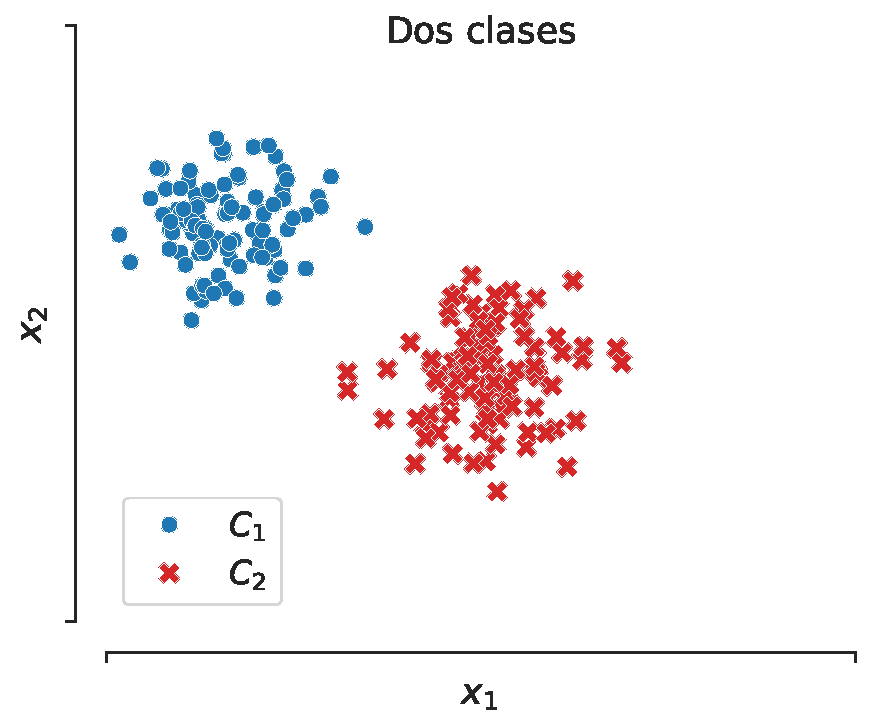
\includegraphics[width=0.8\textwidth]{img/cap2_dosclases}\\
    \captionof{figure}{Ejemplo de datos, los puntos\\ en azul pertenecen a $\mathcal{C}_1$, los rojos a $\mathcal{C}_2$.}
    \label{fig:puntos_2d}
\end{minipage}

\vspace{1cm}
La superficie de decisión queda definida por $y(x)=0$, si $x\in\R^D$, entonces la superficie de decisión corresponde a un hiperplano de dimensión $D-1$.

Sean $x_1,x_2$ dos puntos en la superficie de decisión, entonces se cumple lo siguiente:

\begin{align}
    0 &= y(x_1) - y(x_2) \nonumber\\
      &= \theta^Tx_1 + w - \theta^Tx_2 - w \nonumber\\
      &= \theta^T(x_1-x_2)
\end{align}

Esto muestra que $\theta$ es ortogonal a cualquier vector que esté contenido dentro del hiperplano de decisión, esto nos dice que el vector $\theta$ controla la inclinación del hiperplano.

Por otro lado, si $y(x)=0$:

\begin{equation}
    \frac{\theta^Tx}{\left \| \theta \right \|} = -\frac{w}{\left \| \theta \right \|}
\end{equation}

Esto muestra que la distancia normal de un punto $x$ en la superficie de decisión al origen está dada por el parámetro $w$.

Más aun $y(x)$ da una media con signo sobre cuanto es la distancia perpendicular $r$ entre el punto $x$ y la superficie de decisión. Dado cualquier punto $x$, este puede ser descompuesto en su proyección ortogonal sobre la superficie de decisión $x_{\bot}$ y la componente restante respecto al vector $\theta$, de forma que:

\begin{align}
    x &= x_{\bot}+r\frac{\theta}{\left \| \theta \right \|}\\
    y(x) &= \theta^Tx+w\\
    &= \theta^Tx_{\bot} + r\frac{\theta^T\theta}{\left \| \theta \right \|} + w\\
    \Rightarrow \quad r &= \frac{\theta^T+w}{\left \| \theta \right \|} 
    = \frac{y(x)}{\left \| \theta \right \|}
\end{align}

\newpage
\subsubsection{Caso multi clase}

Si se tienen $K$ clases $\mathcal{C}_k$ distintas, un enfoque posible para abordar el problema de clasificación es considerar $K$ discriminantes lineales.

\begin{equation}
    y_k(x) = \theta_k^Tx + w_k, \quad k=1,\ldots,K
\end{equation}

Donde $x$ será asignado a la clase $\mathcal{C}_k$ si y solo si $y_k(x) > y_j(x),\quad \forall j\neq k$, es decir:

\begin{equation}
    \mathcal{C}(x) = \underset{k}{\argmax}\hspace{1mm} y_j(x)
\end{equation}

\subsubsection{Clasificación con mínimos cuadrados}

Ya planteado el modelo, la pregunta que queda por responder pasa a ser como determinar $\theta$ y $w$, dado los métodos presentados en las clases anteriores el enfoque de mínimos cuadrados parece una respuesta natural a este problema, en primer lugar se introducirá un poco de notación para plantear el problema de una forma cómoda.

Dadas $\{\mathcal{C}_k\}_{k=1}^K$ clases distintas y un punto $x$ usaremos el vector $t\in\{0,1\}^K$ para codificar la pertenencia de $x$ a una clase especifica, por ejemplo: si $x\in\mathcal{C}_j$ entonces el vector $t$ asociado estará compuesto 

\begin{equation}
    x\in\mathcal{C}_j \Leftrightarrow t_j=1 \wedge t_i=0, \quad i\neq j
\end{equation}

esta codificación también es conocida como 'one-hot'.

Cada clase $\mathcal{C}_k$ posee su propio modelo lineal:

\begin{equation}
    y_k(x) = \theta_k^Tx + w_k \nonumber
\end{equation}

El sistema puede ser reescrito de forma matricial como:

\begin{equation}
    y(x) = \tilde{\Theta}^T\tilde{x}
\end{equation}

Donde la $K$-esima columna de $\tilde{\Theta}$ es un vector de $D+1$ dimensiones definido por $\tilde{\theta}=(w_k, \theta_k^T)^T$ y $\tilde{x}=(1,x^T)^T$ corresponde al vector $x$ aumentado. De esta forma un punto $x$ será asignado a la clase que tenga mayor $y_k=\tilde{\theta}_k^T\tilde{x}$.

Considerando un conjunto de entrenamiento $\{x_n,t_n\}_{n=1}^N$, definimos las siguientes matrices:

\begin{align}
    T &= [t_1, t_2,\ldots, t_N]^T\\
    \tilde{X} &= [\tilde{x}_1, \tilde{x}_2, \ldots, \tilde{x}_N ]^T
\end{align}

Finalmente para determinar los coeficientes de $\tilde{\Theta}$, minimizamos la suma de los errores cuadráticos de forma similar al problema de regresión, la función de costo puede ser escrita de la siguiente manera:

\begin{equation}
    E_D(\tilde{\Theta}) = Tr\{(\tilde{\Theta}\tilde{X}-T)^T(\tilde{\Theta}\tilde{X}-T)\}
\end{equation}

Donde $Tr$ corresponde al operador traza, al derivar e igualar a 0 la expresión (92), la solución es:

\begin{equation}
    \tilde{\Theta} = (\tilde{X}^T\tilde{X})^{-1}\tilde{X}T = \tilde{X}^*T
\end{equation}

Donde $\tilde{X}^*$ denota la pseudo-inversa de la matriz $\tilde{X}$, finalmente la solución es:

\begin{equation}
y(x) = T^T(\tilde{X}^*)\tilde{x}
\end{equation}

El problema con este enfoque es que mínimos cuadrados es muy sensible a la presencia de puntos aislados, dada la penalización cuadrática, los puntos lejanos al promedio de los datos tiene una influencia mucho mayor, lo que puede empeorar considerablemente los resultados.


\begin{figure}[H]
    \centering
    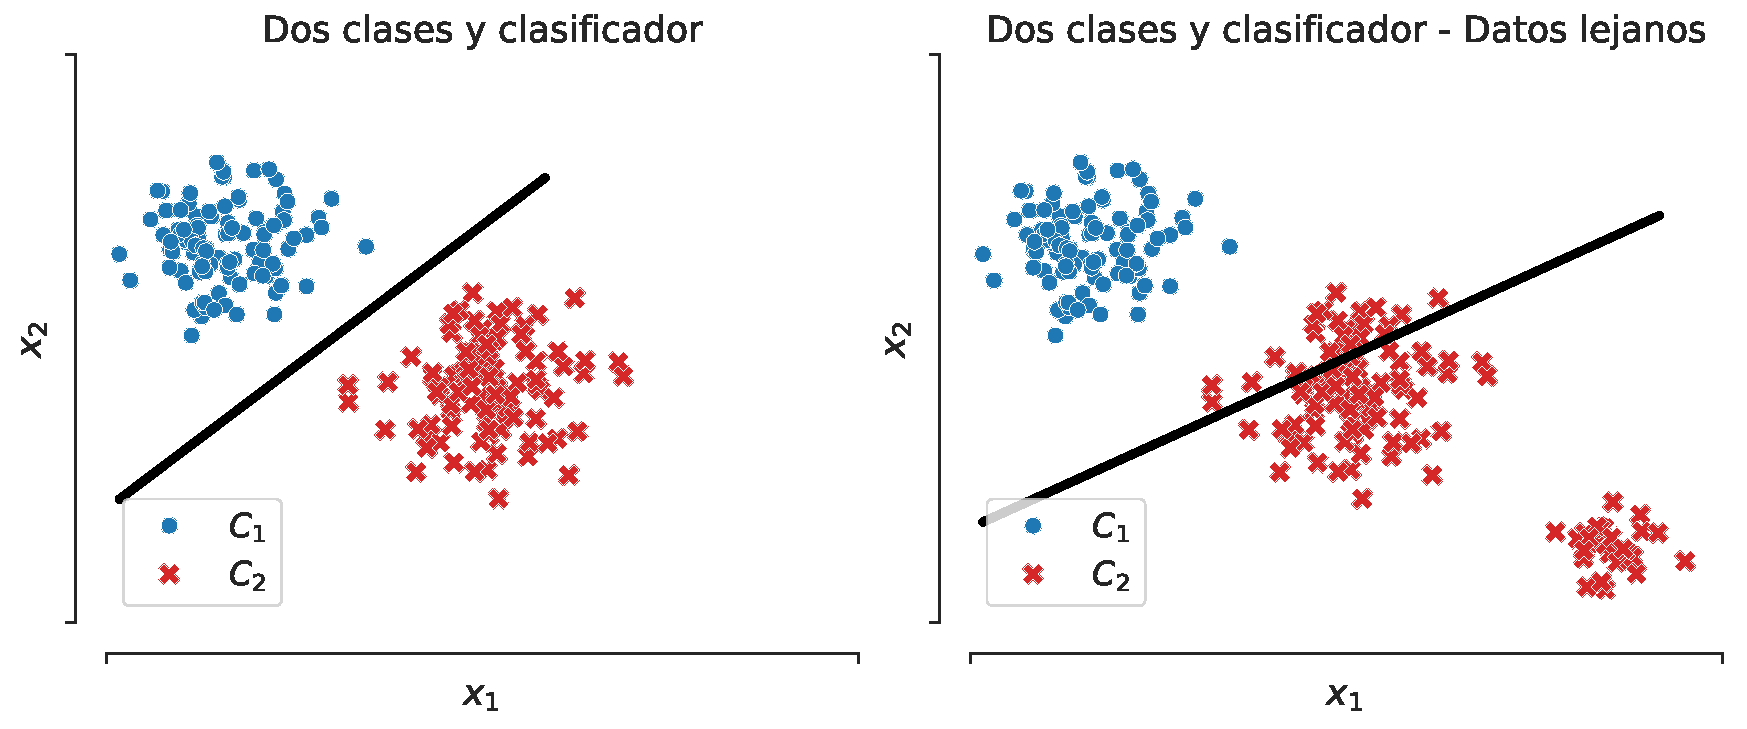
\includegraphics[width=0.7\textwidth]{img/cap2_dosclases_clasificador.pdf}\\
    \caption{Ejemplo ilustrativo sobre como los puntos lejanos pueden afectar negativamente los resultados.}
    \label{fig:clasif_mse}
\end{figure}

\subsubsection{Discriminante lineal de Fisher}

Una forma de ver un modelo de clasificación es en termino de reducción de dimensionalidad. Consideremos el caso en que hay 2 clases y un vector $x\in R^D$ que proyectamos a 1 dimensión de la siguiente manera:

\begin{equation}
    y = \theta^Tx
\end{equation}

Si definimos un umbral $w$, asignamos $x$ a $\mathcal{C}_1$ si $y\geq-w$ y $x$ a $\mathcal{C}_2$ en el caso contrario, recuperamos el modelo lineal que se discutido a través de esta capítulo.

En general al proyectar $D$ dimensiones a 1 se pierde gran cantidad de la información, esto se expresa en el hecho que clases claramente separadas en el espacio $D$-dimensional pueden traslaparse al ser proyectadas a 1 dimensión. Sin embargo al ajustar las componentes de $\theta$, podemos seleccionar una proyección que maximice la separación entre clases.

Para comenzar sean $N_1 = |\mathcal{C}_1|$ y $N_2 = |\mathcal{C}_2|$, con esto calculamos los promedios por clase.

\begin{equation}
    \text{m}_1=\frac{1}{N_1}\sum_{n\in\mathcal{C}_1}x_n
    \quad\quad\quad
    \text{m}_2=\frac{1}{N_2}\sum_{n\in\mathcal{C}_2}x_n
\end{equation}

La medida más simple de separación entre las clases cuando son proyectadas sobre $\theta$ es la separación entre los promedios de clase, esto sugiere elegir un $\theta$ que maximice la siguiente expresión

\begin{equation}
    m_1 - m_2 = \theta^T(\text{m}_1-\text{m}_2)
\end{equation}

Donde $m_k= \theta^T\text{m}_k$ corresponde al promedio de la clase $\mathcal{C}_k$ proyectado sobre $\theta$. Esta expresión puede ser arbitrariamente grande si escalamos $\theta$, para evitar imponemos que $\left \| \theta \right \|_2=1$. Usando multiplicadores de Lagrange para optimizar el problema restringido se llega a que $\theta\propto(\text{m}_1-\text{m}_2)$. El problema con esta solución es que pueden existir 2 clases bien separadas en el espacio $D$-dimensional, pero al proyectar los datos sobre la recta que une sus promedios, las proyecciones de cada clase se traslapen.

\begin{figure}[H]
    \centering
    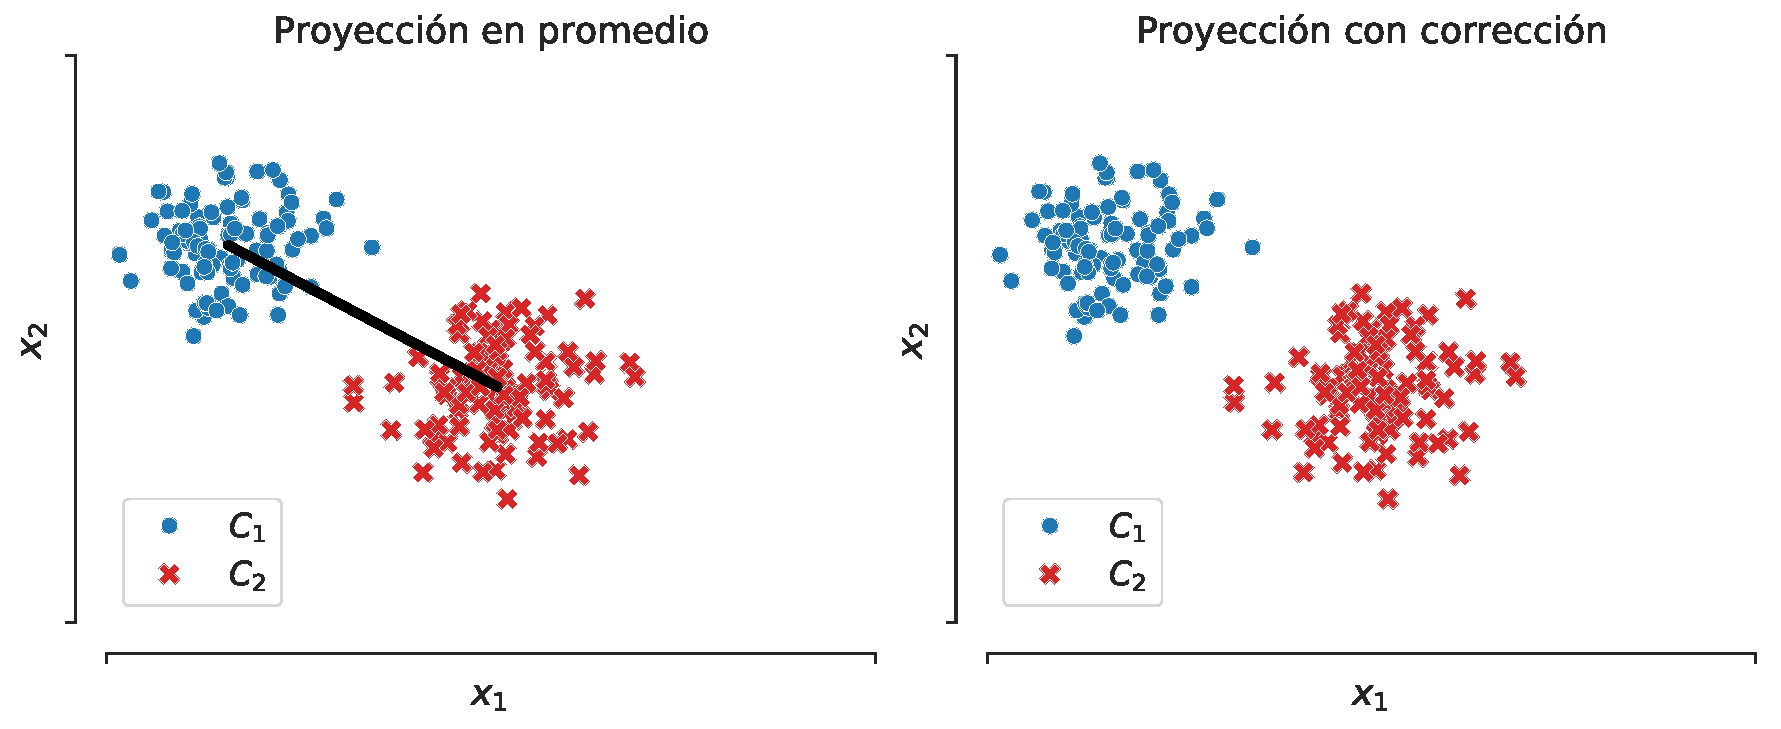
\includegraphics[width=0.7\textwidth]{img/cap2_dos_clases_proyeccion.pdf}\\
    \caption{(a) Resultado obtenido al proyectar sobre la recta que une los promedios de cada clase. (b) Resultado al considerar una corrección que considera minimizar la dispersión entre clases.}
    \label{fig:ej_fda}
\end{figure}

Para resolver este problema Fisher propuso maximizar una función que de como resultado una gran separación entre clases distintas, pero que al mismo tiempo minimice la separación dentro de una misma clase, de esta forma el traslape entre clases disminuye. 

Definimos la varianza dentro una clase como:

\begin{align}
    s_k^2 &= \sum_{n\in \mathcal{C}_k}(\theta^T(x_n-\text{m}_k))^2\\
    &= \sum_{n\in \mathcal{C}_k}(y_n-m_k)^2
\end{align}
Con esto se define la nueva función objetivo de la siguiente manera:

\begin{equation}
J(\theta) = \frac{m_1-m_2}{s_1^2+s_2 ^2}
\end{equation}

Podemos usar la ecuaciones descritas anteriormente para escribir $J(\theta)$ de forma explicita respecto a $\theta$.

\begin{equation}
    J(\theta) = \frac{\theta^TS_B\theta}{\theta^TS_W\theta}
\end{equation}

Donde $S_B$ es la matriz de covarianza entre clases dada por:

\begin{equation}
    S_B = (\text{m}_1-\text{m}_2)(\text{m}_1-\text{m}_2)^T
\end{equation}

$S_W$ es la matriz total de covarianza dentro de clases, dada por:

\begin{equation}
    S_W = \sum_{n\in \mathcal{C}_1}(x_n-\text{m}_1)(x_n-\text{m}_1)^T+
    \sum_{n\in \mathcal{C}_2}(x_n-\text{m}_2)(x_n-\text{m}_2)^T
\end{equation}

Al derivar $J(\theta)$ se encuentra que la función es maximizada cuando:

\begin{equation}
    (\theta^TS_B\theta)S_W\theta = (\theta^TS_W\theta)S_B\theta
\end{equation}

Por la definición de $S_B$, vemos que $S_B\theta$ es co-lineal con $(\text{m}_1-\text{m}_2)$. Más aun no es importante la norma de $\theta$, solo interesa la orientación, por esta razón descartamos los escalares $(\theta^TS_B\theta)$ y $(\theta^TS_W\theta)$, al despejar $\theta$ vemos que la solución es:

\begin{equation}
    \theta \propto S_W^{-1}(\text{m}_1-\text{m}_2)
\end{equation}
\newpage
\subsection{Clasificación No Lineal}

\subsubsection{El Perceptrón}

El perceptrón de Rosenblatt es un modelo de clasificación binario que tuvo mucha importancia en el área de reconocimiento de patrones. El modelo consiste en una función no-lineal fija usada para transformar $x$ en un vector de características $\phi(x)$, que luego es usado para generar un modelo lineal generalizado de la siguiente forma:

\begin{align}
    y(x) &= f(\theta^T\phi(x))\\
    f(a) &= \left\{\begin{matrix}
    +1,\quad a\geq 0\\
    -1,\quad a<0
    \end{matrix}\right.
\end{align}

Típicamente el vector $\phi(x)$ contiene un intercepto para la recta, es decir $\phi_0\equiv1$. El modelo asigna $x$ a la clase $\mathcal{C}_1$ si $y(x)=+1$ y asignará $x$ a la clase $\mathcal{C}_2$ cuando $y(x)=-1$.

Para encontrar el vector $\theta$ suele usarse un criterio basado en los datos que fueron clasificados incorrectamente llamado el criterio del perceptrón, este puede deducirse notando que se quiere encontrar un vector de pesos $\theta$ tal que para los $x\in\mathcal{C}_1$ cumpla $\theta^T\phi(x) > 0$ y para los $x\in\mathcal{C}_2$ cumpla $\theta^T\phi(x) < 0$, usando el hecho que $y(x)\in\{1,-1\}$, ambas condiciones pueden ser cubiertas por la expresión:

$$\theta^T\phi(x)y(x) > 0,\quad \forall x \in \mathcal{C}_1\cap\mathcal{C}_2$$

El criterio del perceptrón asocia a los puntos clasificados correctamente 0 error y a los puntos mal clasificados error $-\theta^T\phi(x)y(x)$, de esta forma si denotamos como $\mathcal{M}$ el conjunto de puntos mal clasificados, se debe minimizar la siguiente función objetivo:

$$ E_p(\theta) = -\sum_{i\in\mathcal{M}}\theta^T\phi(x_i)y(x_i) $$

Para minimizar esta función se usa descenso de gradiente estocástico, las actualizaciones son de la siguiente manera:

\begin{align}
    \theta^{\tau+1} &= \theta^\tau - \eta \nabla E_p(\theta)\\
    &= \theta^\tau + \eta \phi(x_n)y(x_n)
\end{align}

La constante $\tau$ corresponde a un entero que indexa las iteraciones. Por otra lado $\eta$ es una constante que se conoce como tasa de aprendizaje, dado que la función del perceptŕon $y(x)=y(x,\theta)$ no cambia si se multiplica $\theta$ por una constante cualquiera, sin perdida de generalidad podemos asumir que $\eta=1$. Es importante notar que al actualizar el vector $\theta$, el conjunto de puntos mal clasificados $\mathcal{M}$ va a cambiar.

La interpretación del algoritmo usado para ajustar el perceptrón es simple, se recorre el conjunto de puntos de entrenamiento $\{x_n\}_{n=1}^N$, si el punto $x_n$ fue clasificado correctamente el vector de pesos de mantiene igual, por otro lado si $x_n$ fue clasificado incorrectamente, el vector $\theta^\tau$ es actualizado según (89).
\newpage
\subsubsection{Clasificación Probabilista}

Los modelos que hemos mencionado anteriormente son de tipo discriminativo, es decir modelan directamente la probabilidad condicional $\mathbb{P}(\mathcal{C}_k|x)$, que da la probabilidad de pertenencia a una clase dado un dato.

Otro paradigma más poderoso a considerar es un enfoque generativo en el cual modelamos $\mathbb{P}(x|\mathcal{C}_k)$ junto con un prior $\mathbb{P}(\mathcal{C}_k)$ para las clases, luego podemos calcular la densidad posterior usando el Teorema de Bayes.

\begin{equation}
    \mathbb{P}(\mathcal{C}_k|x) = \frac{\mathbb{P}(x|\mathcal{C}_k)\mathbb{P}(\mathcal{C}_k)}{\mathbb{P}(x)}
\end{equation}

Considere el siguiente desarrollo, para el caso con 2 clases:

\begin{align}
    \mathbb{P}(\mathcal{C}_1|x) &= \frac{\mathbb{P}(x|\mathcal{C}_1)\mathbb{P}(\mathcal{C}_1)}{\mathbb{P}(x)}\\
    &= \frac{\mathbb{P}(x|\mathcal{C}_1)\mathbb{P}(\mathcal{C}_1)}{\mathbb{P}(x|\mathcal{C}_2)\mathbb{P}(\mathcal{C}_2)+\mathbb{P}(x|\mathcal{C}_1)\mathbb{P}(\mathcal{C}_1)}\\
    &=\frac{1}{1+\frac{\mathbb{P}(x|\mathcal{C}_1)\mathbb{P}(\mathcal{C}_1)}{\mathbb{P}(x|\mathcal{C}_2)\mathbb{P}(\mathcal{C}_2)}}\\
    &=\frac{1}{1+\exp(-a)} = \sigma(a)\\
\end{align}

Donde $a = \ln(\frac{\mathbb{P}(x|\mathcal{C}_1)\mathbb{P}(\mathcal{C}_1)}{\mathbb{P}(x|\mathcal{C}_2)\mathbb{P}(\mathcal{C}_2)})$.

\begin{itemize}
    \item La función logística está se define como $\sigma(a) = \frac{1}{1+e^{-a}}$.
    
    \item Tiene propiedades útiles como $\sigma(-a)=1-\sigma(a)$ y $\frac{d}{da}\sigma(a)=\sigma(a)(1-\sigma(a))$
    
    \item La inversa de la función logística se conoce como logit y es definida por $a(\sigma)=\ln(\frac{\sigma}{1-\sigma})$
\end{itemize}

Para el caso multi-clase, se puede hacer un desarrollo similar:

\begin{align}
    \mathbb{P}(\mathcal{C}_i | x) &= \frac{\mathbb{P}(x | \mathcal{C}_i)\mathbb{P}(\mathcal{C}_i)}{\sum_{j\neq i}\mathbb{P}(x | \mathcal{C}_j)\mathbb{P}(\mathcal{C}_j)}\\
    &= \frac{\exp(a_i)}{\sum_{j\neq i}\exp(a_j)}\\
    a_i &= \mathbb{P}(x | \mathcal{C}_i)\mathbb{P}(\mathcal{C}_i)
\end{align}

La función que aparece se conoce como softmax y corresponde a una generalización de la función logística a más dimensiones, adicionalmente tiene la propiedad de ser una aproximación suave de la función máximo.

\newpage

\noindent{\textbf{-Ejemplo:}} Normal class-conditional densities

Suponemos que las densidades condicionales de clase distribuyen como una normal multivariada, $p(x|\mathcal{C}_k) \sim \mathcal{N} (\mu_k,\Sigma)$ :

\begin{align}
p(x|\mathcal{C}_k)&=\frac{1}{(2\pi)^\frac{D}{2}|\Sigma|^\frac{1}{2}}\exp(-\frac{1}{2}(x-\mu_k)^T\Sigma^{-1}(x-\mu_k))\\
\Rightarrow \quad a &= \ln(\exp(-\frac{1}{2}(x-\mu_1)^T\Sigma^{-1}(x-\mu_1) +\frac{1}{2}(x-\mu_2)^T\Sigma^{-1}(x-\mu_2)))\\
&= \theta^Tx+w
\end{align}

Donde:

\begin{align}
\theta &= \Sigma^{-1}(\mu_1-\mu_2)\\
w &= \frac{1}{2}(\mu_1^T\Sigma^{-1}\mu_1+\mu_2^T\Sigma^{-1}\mu_2)
+\ln(\frac{p(\mathcal{C}_1)}{p(\mathcal{C}_1)})\\
\Rightarrow \quad p(\mathcal{C}_k|x) &= \sigma(\theta^Tx+w)
\end{align}

¿Como ajustar los parámetros de las condicionales a la clase y priors respectivamente?

\begin{itemize}
    \item\textbf{Parámetros:}
    \begin{align}
    p(\mathcal{C}_1)&=\pi \quad \Rightarrow \quad p(\mathcal{C}_2)=1-\pi\\
    p(x|\mathcal{C}_k) &= \mathcal{N}(\mu_k,  \Sigma); k=1,2
    \rightarrow \mu_1,\mu_2,\Sigma
    \end{align}
    
    \item\textbf{Datos:}
    \begin{align}
    T&=(t_1,t_2,\ldots,t_N) \in \{0,1\}^N\\
    X&=(x_1,x_2,\ldots,x_N)
    \end{align}
    
    \item\textbf{Likelihood:}
    
    Se recuerda que $p(x,\mathcal{C}_k)=p(x|\mathcal{C}_k)p(\mathcal{C}_k)=p(\mathcal{C}_k)\mathcal{N}(x|\mu_k,\Sigma)$, se procede a calcular la función de verosimilitud de los datos:
    
    \begin{align}
    p(X,T|\pi,\mu_1,\mu_2,\Sigma) &= \prod_{i=1}^{N}p(x_i,t_i|\pi,\mu_1,\mu_2,\Sigma)\\
    &= \prod_{i=1}^{N}p(x_i,\mathcal{C}_1)^{t_i}p(x_i,\mathcal{C}_0)^{1-t_i}\\
    &= \prod_{i=1}^{N}(\pi\mathcal{N}(x_i|\mu_1,\Sigma))^{t_i}
    ((1-\pi)\mathcal{N}(x_i|\mu_2,\Sigma))^{1-t_i}
    \end{align}
    
    Más facil que el likelihood, es log-likelihood:
    
    \begin{equation}
    \log(L) := \sum_{i=1}^{N}t_i(\log(\pi)+\log(\mathcal{N}(x_i|\mu_1,\Sigma)))+(1-t_i)(\log(1-\pi)+\log(\mathcal{N}(x_i|\mu_2,\Sigma)))
    \end{equation}
    
    \newpage
    \noindent \textbf{1)}Derivada con respecto a $\pi$:
    
    \begin{align}
    \frac{\partial\log(L)}{\partial\pi} &= \sum_{i=1}^N \frac{t_i}{\pi}+\frac{1-t_i}{1-\pi}=0\\
    \Rightarrow \quad & (i-\pi)\sum_{i=1}^Nt_i = \pi\sum_{i=1}^N(1-t_i)\\
    \Rightarrow \quad & \sum_{i=1}^Nt_i=\pi N \quad\Rightarrow\quad \pi = \frac{\sum_{i=1}^Nt_i}{N} = \frac{N_1}{N_1+N_2}
    \end{align}
    
    Observamos que el valor encontrado para $\pi$ corresponde al promedio de las clases.
    
    \noindent \textbf{2)}Derivada con respecto a $\mu_1$:
    
    \begin{align}
    \frac{\partial\log(L)}{\partial\mu_1} &= \sum_{i=1}^N t_i
    \frac{\partial}{\partial \mu_1}(-\frac{1}{2}(x_i-\mu_1)^T\Sigma^{-1}(x_i-\mu_1))\\
    &= \sum_{i=1}^N t_i(\Sigma^{-1}(x_i-\mu_1)) =
    \Sigma^{-1}\sum_{i=1}^N t_i(x_i-\mu_1) = 0\\
    \Rightarrow\quad & \sum_{i=1}^Nt_ix_i= \mu_1\sum_{i=1}^N t_i
    \quad\Rightarrow\quad \mu_1 = \frac{1}{N_1}\sum_{i=1}^Nt_ix_i
    \end{align}
    
    De forma análoga:
    \begin{equation}
    \mu_2 = \frac{1}{N_2}\sum_{i=1}^N(1-t_i)x_i
    \end{equation}
    
\end{itemize}

\subsubsection{Regresión Logística v/s Modelo Generativo}

Los supuestos hechos sobre el modelo generativo resultaron en:

\begin{equation}
p(\mathcal{C}_1|x) = \sigma(w^Tx) = \frac{1}{1+e^{-w^Tx}}
\end{equation}

Encontrar $w$ de forma directa es mucho más fácil que ajustar todos los parámetros del modelo generativo.

Para dejar este punto en claro, se calculará la verosimilitud de la regresión logística con datos $\{x_i,y_i\}_{i=1}^N$, para hacer la notación más compacta denotamos $\sigma_i = \sigma(w^Tx_i)$.


\begin{align}
p(y_{1:N}|x_{1:N},w) &= \prod_{i=1}^{N}p(y_i|x_i,w)\\
&= \prod_{i=1}^{N}\sigma_i^{y_i}(1-\sigma_i)^{1-y_i}\\
NLL &= -\log(p(y_{1:N}|x_{1:N},w))\\
&= -\sum_{i=1}^N y_i\log(\sigma_i) + (1-y_i)\log(1-\sigma_i)
\end{align}

Se procede a calcular el gradiente de $NLL$ respecto a $w$:

\begin{align}
\nabla_w NLL &= -\sum_{i=1}^N y_i\frac{\sigma_i(1-\sigma_i)}{\sigma_i}x_i
+ (1-y_i)\frac{-\sigma_i(1-\sigma_i)}{\sigma_i}x_i\\
&= -\sum_{i=1}^N y_i(1-\sigma_i)x_i - (1-y_i)\sigma_ix_i\\
&= \sum_{i=1}^N (\sigma_i-y_i)x_i
\end{align}











